\section{Apresentação dos Resultados Obtidos}

Levando em consideração os resultados obtidos através da aplicação de todos os cenários de testes descritos acima sob os serviços desenvolvidos neste trabalho, é possível afirmar que a utilização da Unidade de Resposta Audível na realização dos atendimentos de primeiro nível, tem potencial para reduzir parte dos atendimentos destinados aos serviços obter 2ª via de conta, informar falta de água e solicitar restabelecimento da ligação de água, e também contribuir com a padronização dos atendimentos e a redução dos custos.

Com a suíte de testes automatizados desenvolvida é possível garantir o correto funcionamento da integração entre os sistemas GSAN e Asterisk proposta neste trabalho e contribuir com a comunidade de software livre agregando uma nova funcionalidade de automação dos serviços obter 2ª via de conta, informar falta de água e solicitar restabelecimento da ligação de água, como também uma nova suíte de testes automatizados focados na verificação da integração.
 
 %observando os percentuais atingidos com base na média descrita dos principais %Serviços do Atendimento ao Público, notamos que a solução proposta é capaz de %reduzir em até 20,46\%, dos registros de atendimentos diários, conforme visto %abaixo na figura \ref{figura:eficienciaServicos}:	

%\begin{figure}[!htb]
%	\centering
%	\caption{Gráfico de avaliação dos serviços automatizados}
%	\label{figura:eficienciaServicos}	
%	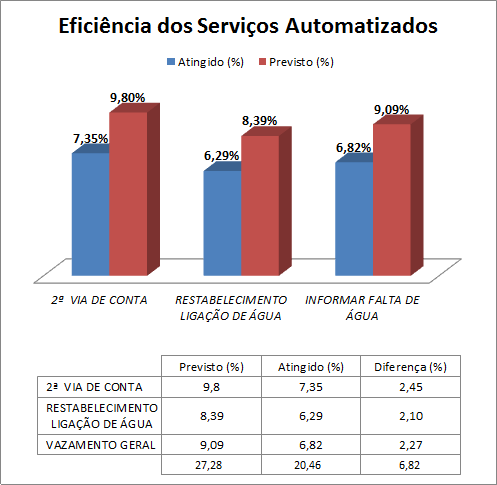
\includegraphics{figuras/eficiencia_servicos.png}
%	\legend {\fontsize{10}{12}\selectfont {Fonte: Autoria Própria}.}
%\end{figure}

